
\section{Stability principle}
\label{sec:II}
%Firstly we consider the trap mirror as a suspended mirror located at the end of a Fabry-Perot cavity. 
%Dual carrier approach for mirror position control is based on the use of a strong (carrier) and a weak
%(subcarrier) field created to form two optical springs in such a way to have a stable system when 
%summed to the mechanical spring. %An additionally couple of beams need to be used for the angular control.

An optically detuned Fabry-Perot cavity naturally leads to a linear coupling between intra-cavity power and 
mirror position. Depending on the sign of the detuning, this coupling creates an optical spring which
is either statically stable or unstable. Due to the time delay in the optical field build-up, the optical spring 
restoration force is slightly delayed. This leads to a dynamically unstable spring for the statically stable case
and a dynamically stable spring for the statically unstable case. Corbitt et. al. \cite{Corbitt07} demonstrated that by adding a second, frequency-shifted optical field (sub-carrier) with a different detuning and power, a statically and dynamically stable optical spring can be achieved. The dual-carrier scheme has been used to optically trap a gram-scale mirror, controlling its longitudinal degree of freedom.
%thus creating an optical trap for the length degree of freedom of the mirror. 
Moreover, the damping of the optical spring can be controlled by adjusting the detuning of both carrier and sub-carrier and their relative amplitudes. This naturally allows for efficient cooling of the degree of freedom seen by the optical spring. In contrast to a mechanical spring, this damping does not introduce intrinsic losses, and thus does not contribute to the thermal noise.

This technique can be extended to alignment degrees of freedom. By duplicating the Corbitt et al. approach for trapping 
with a second, different, optical axis and a different beam spot on the controlled mirror, it is possible to control the angular 
degree of freedom with radiation pressure alone.
%, thus by-passing the Sidles-Sigg instability.

To be able to understand the stability of multi-dimensional opto-mechanical systems, we first recall the simple driven damped mechanical oscillator. From there we will stepwise increase the complexity by adding optical springs and additional degrees of freedom. 
%\tcr{Following we recall some of the features of a driven mechanical damped oscillator, we introduce the mathematical form of a optical spring and its relation with a mechanical oscillator in terms of control system model.}

%This lead us to the use of a two carrier scheme for the control of a single degree of
%freedom and to a double two carriers scheme for the control of two degrees of freedom.

%%%%%%%%%%%%%%%%%%%%%%%%%%%%%%%%%%%%%%%%%%%%%%%%%%%%%%%%%%%%%%
\subsection{Damped mechanical oscillator stability}
%%%%%%%%%%%%%%%%%%%%%%%%%%%%%%%%%%%%%%%%%%%%%%%%%%%%%%%%%%%%%%

Although the damped mechanical oscillator is a well known system, we will take it as a starting point to make the reading clearer. Our goal is to describe the mechanical oscillator in the language of control theory, which allows us to understand the stability of the system from a different point of view. This approach can then be naturally extended to include the effect of additional optical springs. 

The motion of a harmonic oscillator of mass $m$, spring constant $k_m$ and velocity damping $b$, driven by the external force $F_{ext}$, can be expressed as \cite{Saulson90}:
\begin{eqnarray}
\label{eqn:motion}
m\ddot{x}=-k_m x-b\dot{x}+F_{ext}
\end{eqnarray}
$b$ is also called the viscosity coefficient. Often the damping rate $\Gamma=b/(2 m)$ is used instead.
Traditionally the equation of motion \ref{eqn:motion} is directly used to get the system's position response $x$ when applying the external force $F_{ext}$. The resulting transfer function is
%For such a purpose and for completeness  we can describe the mechanical oscillator in two different way. 
%Both ways are self-consistent.
%One way is to consider the system as a mass with a mechanical spring that moves of the quantity $x$ when subjected at
%the force $F_{ext}$. The law that link the output $x$ and the input $F_{ext}$ of the system is
%given by the transfer function which can be directly obtained by the equation of motion (\ref{eqn:motion}):
%We consider such a system as free-test mass 
%\begin{figure}[htbp]
%	\centering
		%\includegraphics[width=6cm]{./images/Spring_add.eps}
%		\includegraphics[width=5cm]{./images/block_1.eps}
%	\caption{bla bla bla}
%	\label{cavity_k}
%\end{figure}

%That leads to the following transfer function:
\begin{eqnarray}
\label{eqn:TF}
G=\frac{x}{F_{ext}}=\frac{1}{-m\Omega^2+k_m+ib\Omega}                                                 %=\frac{1}{ms^2+b s+k_m}
\end{eqnarray}
with $\Omega$ being the angular frequency of the motion.
% and $s=i\Omega$ being a complex variable. % and $\Gamma=b/m$ is the damping rate. 

Alternatively we can describe a damped mechanical oscillator as a feedback system,  with the plant being just a free-test mass described by the transfer function 
$M=x/F_{ext}=-1/m\Omega^2$,
%Another way that can be used to describe a damped mechanical oscillator is to consider it as
%a feedback system where its plant is just a free-test mass described by the transfer function 
%$M=x/F_{ext}=-1/m\Omega^2$, 
obtained directly from the equation of motion of a free test-mass. 
The control filter of the feedback loop is the mechanical spring, which takes the mass displacement $x$ as input and acts on the plant with the control signal, or force, $F_K$, which is subtracted from the external force $F_{ext}$.
The transfer function of the control filter is $K_M=F_{K}/x=k_m+ib\Omega$. In this picture we can now calculate the closed loop transfer function and obtain the same expression as in equation \ref{eqn:TF}:
\begin{eqnarray}
\label{eqn:TF_fm}
G=\frac{M}{1+K_M M}=
%\frac{\frac{-1}{m\Omega^2}}{1-\frac{K_M}{m\Omega^2}}=
\frac{1}{-m\Omega^2+k_m+ib\Omega}
\end{eqnarray}
where $OL_M=-K_M  M = (k_m+ib\Omega)/m\Omega^2$ describes the open loop transfer function of the system.

%\begin{figure}[htbp]
%	\centering
%		%\includegraphics[width=6cm]{./images/Spring_add.eps}
%		\includegraphics[width=8cm]{./images/blocks}
%	\caption{{(Left)} A damped mechanical oscillator seen as system subjected to the external 
%	force $F_{ext}$ and corresponding displacement $x$ as output.
%	{(Right)} A damped mechanical oscillator seen as a closed-loop system, where the plant $M$
%	is a free-mass, the output is the displacement $x$ which is fed-back to the system through the elastic force $F_k= -K_M \cdot x$ and the input is $F_{ext}-F_{k}$.}
%	\label{fig:blocks}
%\end{figure}

\subsubsection*{Stability}
We can now check for the stability of the system in both pictures.
%The stability of the system related to the two different descriptions can be evaluated in a different manner.
%While the stability in the first description can be evaluated by looking at the poles of its transfer function, the latter
%offers the additional chance to look at its open loop transfer function $M\cdot K_M$ to evaluate its stability.
We recall from literature that the stability of a system described by its transfer function $G$ can be evaluated looking at the poles 
of its transfer function in the s-plane ($s=i\Omega$) \cite{Greensite70}. In particular a system is stable only if its transfer function's poles have
a negative real part,  and the multiplicity of poles on imaginary axis is at most 1.
The transfer function in equation \ref{eqn:TF} has the following poles:
\begin{eqnarray}
\label{eqn:poles}
i\Omega=-\frac{b}{2m}\pm\sqrt{\frac{b^2}{4m^2}-\omega_0^2},
\end{eqnarray}
where $\omega_0^2=k_m/m$ is the resonant frequency of the pendulum. 
%Comparing the damping rate $\Gamma=b/2m$ with the resonance frequency $\omega_0$ we understand the type of poles presents in $G$. If  $\Gamma>\omega_0$ then the poles are real and negative (over-damping), 
%if $\Gamma<\omega_0$ than the poles are complex conjugate at negative real part (under-damping),
%and if $\Gamma=\omega_0$ the system has two equal poles with negative real part (critically-damping).
The value of the damping rate $\Gamma=b/2m$ compared to $\omega_0$ determines whether the system is over-damped, under-damped or critically-damped. But since  $\Gamma$ (or $b$) is always positive, 
the real part of the poles is always negative. The system is thus always stable. 
%Here we want to point out that what ever cases we consider
%a damped mechanical oscillator shows poles with negative real component as $b$ and $k_m$ are in any cases positive, thus the system is always stable. 

From the control theory point of view, the stability can also be evaluated with no loss of generality by considering the open loop transfer function $OL_M= (k_m+ib\Omega)/m\Omega^2$ and applying, for example, the Bode stability criterion \cite{Franklin94}. The positivity of $b$ guarantees an always positive phase margin and therefore stability.
In the reminder of this work, for simplicity, we will test the stability of the control scheme using the Bode graphical method.

%as long as we consider the open loop transfer function $OL_M$. In this case the stability can be evaluated by using the %Nyquist criterion \cite{} by considering the plot of the open loop transfer function
%in the complex plane \cite{}

%can be evaluated by using the Nyquist criterion by considering the plot of the open loop transfer function
%in the complex plane \cite{}.


\subsection{Optical spring: a classical model}
Next, we look at an optical spring.
We start with a Fabry-Perot  cavity of length 
$L_0$, frequency detuning $\delta$, amplitude transmittance coefficients $t_1$, $t_2$  and amplitude reflectance coefficients $r_1$, $r_2$ of the input and output cavity mirror respectively. 
The light field inside the cavity builds up and exerts a radiation pressure force on both mirrors.
% In particular if  we calculate the power $P$ of the light inside the cavity, that can be  translated into radiation  pressure force exerted on the end cavity mirror.

We define the propagator $X=r_1r_2e^{-2i\delta\tau}$ and phase factor $Y=e^{-i\Omega\tau}$, with $\tau=L_0/c$ the one-way
travel time of the photon inside the cavity, $k$ is the wave vector of the light field  and $\Omega$ 
is the mechanical frequency of the pendulum. From this we can obtain an elastic force-law for small displacement values $x$, but potentially large detuning from resonance:
\begin{eqnarray}
\label{eqn:Frd}
F_{rad}=F_0-K_{OS}\cdot x + O(x^2),
\end{eqnarray}
where
\begin{eqnarray}
\label{KOS_full_2}
K_{OS}=K_0\left [ \frac{Y^2}{(1-Y^2X)(1-Y^2\overline{X})}  \right ]
\end{eqnarray}
%\begin{eqnarray}
%\label{KOS_full_2}
%\centering
%K_{OS}=-P_0 t^2 r_2^2 \frac{2ike^{-2i\Omega\tau}}{c(1-r_1r_2e^{ikL})(1-r_1r_2e^{-ikL})}\times\nonumber\\
 %\left( \frac{r_1r_2e^{-ikL}}{1-r_1r_2e^{-2i\Omega\tau} e^{-ikL}}-\frac{r_1r_2e^{ikL}}{1-r_1r_2e^{-2i\Omega\tau}e^{ikL}} \right) 
%\end{eqnarray}
is the optical spring constant and $\overline{X}$ is the complex conjugate of $X$. Here $K_0$ is the 
%static (frictionless) 
(mechanical) frequency-independent part of the spring constant:
\begin{eqnarray}
\label{eqn:K0}
K_0=F_0 \cdot 2 i k \cdot (X-\overline{X}),   \quad \mbox{with}\nonumber\\ 
F_0 = P_0 \cdot \frac{2  r_2^2}{c} \cdot \frac{t_1^2}{(1-X)(1-\overline{X})}
%K_0=\eta i \frac{X-\overline{X}}{(1-X)(1-\overline{X})}\quad \mbox{with}\nonumber\\ 
%\eta=P_0 t_1^2 r_2^2\frac{4 k }{c} 
\end{eqnarray}
The expression in equations \ref{KOS_full_2} and \ref{eqn:K0}
is the general expression for $K_{OS}$ up to linear order in $x$. While approximations for this formula have been published before \cite{Barginsky02}, we are not aware of a previous publication providing the full expression.
We address the complete derivation of the optical spring constant $K_{OS}$ in the Appendix \ref{app:A}. There we also show that with the approximations $2\Omega\tau\ll1$ and $2\delta\tau\ll1$  equation \ref{KOS_full_2} is equivalent to the expressions already existing in literature \cite{Barginsky02,Corbitt07}. 

We note that $K_0$ is a real number. Its sign is determined by the imaginary part of $X$. A positive sign is associated with positive detuning ($\delta>0$) and a restoring force (statically stable),  while a negative sign is due to  negative detuning ($\delta<0$) and
leads to a anti-restoring force  (statically unstable).  Also, for small (positive) frequencies $\Omega\tau\ll1$, the sign of the imaginary part of equation \ref{KOS_full_2} is opposite to its real part, leading to positive dynamic feedback for the statically stable case and  negative dynamic feedback for the statically unstable case.

Our next step is to couple the optical spring to a mechanical pendulum. We can treat this as either a damped mechanical oscillator with transfer function $G$, controlled by an optical spring $K_{OS}$, or as a free mass with transfer function $M$, controlled by the total feedback filter $H = K_M + K_{OS}$, see Fig.\ref{fig:blocks2}.
\begin{figure}[htbp]
	\centering
		%\includegraphics[width=6cm]{./images/Spring_add.eps}
		\includegraphics[width=10cm]{./figures/blocks_paper.pdf}
	\caption[Mechanical Oscillator and Feedback]{{
            Mechanical oscillator and feedback systems.
            The mechanical oscillator can be seen as plant ($G$) and the optical
            spring $K_{OS}$ as feedback or alternatively as free test mass
            (plant M) and $H=K_{OS}+K_M$ as feedback. 
	    Both the cases lead to the same closed loop transfer function
            $G_{CL}$ which describes the system as a damped mechanical
            oscillator in presence of the optical spring, subjected to the
            external force $F_{ext}$ and corresponding displacement $x$ as output.}}
	\label{fig:blocks2}
\end{figure}
In both cases we obtain the same closed-loop transfer function, equivalent to the one we would have obtained by
rewriting the equation of motion of a damped mechanical oscillator with an optical spring:
\begin{eqnarray}
\label{eqn:TFco}
G_{CL}=\frac{x}{F_{ext}}=\frac{G}{1+K_{OS} G}=\frac{M}{1+H M}\nonumber\\
=\frac{1}{-m\Omega^2+K_M+K_{OS}}%=\frac{1}{ms^2+b s+k_m}
\end{eqnarray}

The stability of the total system can again be evaluated  by either looking at the poles of the closed-loop
transfer function $G_{CL}$, or looking at the gain and phase margin of the open loop transfer function $OL_{MH}=-H/m\Omega^2$. The latter is generally more convenient. Unless compensated by large mechanical dissipation in $K_M$, the positive dynamic feedback for the statically stable case ($\delta>0$) leads to a dynamically unstable system. 
Intuitively this can be understood as a phase delay in the radiation pressure build-up which is caused by the cavity storage time.
For $\delta<0$ the system is statically unstable.

\subsection{Double Carrier Spring}

The seemingly intrinsic instability of optical springs can be overcome by a scheme 
proposed by Corbitt et al. \cite{Corbitt07}. The carrier is set at a large positive detuning ($\delta>0$, large $\delta/\gamma$). This provides a static restoring force, together with a relatively small dynamic instability (anti-damping). Then a sub-carrier is added at lower power and with a small negative detuning ($\delta<0$, small $|\delta|/\gamma$). The sub-carrier adds sufficient dissipation to stabilize the total optical spring, while leaving the sign of the static restoring force unchanged.
For appropriately chosen parameters of carrier ($c$) and sub-carrier ($sc$) (power $P_0^c$ and $P_0^{sc}$, detuning  $\delta_c$ and $\delta_{sc}$) the resulting total system thus becomes stable.

The spring constant of the total optical spring is simply the sum of the individual spring constants of the carrier and sub-carrier
\begin{eqnarray}
\label{eqn:KOSsum}
K_{OS}=K_{OS}^c+K_{OS}^{sc}
\end{eqnarray}
where the individual springs $K_{OS}^c$ and $K_{OS}^{sc}$ are given by equation \ref{eqn:TFco}.

%Fig.\ref{fig:stability} shows the stability of the trap-system at various values of  sub-carrier power and detuning for fixed carrier settings ($P_0^c=1~{\rm Watt}$, $\delta_c/\gamma = 2$) in our example system.

Conceptually we can think of the dual-carrier optical spring as a physical implementation of a feedback control filter for the mechanical system. With this tool at hand, we can start to analyze the behavior and stability of higher dimensional mechanical systems in the next section.

%\begin{figure}[htbp]
%	\centering
%		\includegraphics[width=9cm]{./images/KMKOSstability}
%	\caption{{Suspension stability region for different sub-carrier detuning ratio $\delta_{sc}/\gamma$ and input power values.
%	The carrier detuning ratio and its power have been set at $\delta_c/\gamma=2$ and $P0_c=1\,$W respectively. 
%	 At $\delta_{sc}/\gamma=0$ or $P0_{sc}=0\,$W only the carrier spring is effective and the system is not stable. The stability
%	 can be recovered only when the sub-carrier beam is injected into the cavity.}}
%	\label{fig:stability}
%\end{figure}


